\documentclass{article}

% Language setting
% Replace `english' with e.g. `spanish' to change the document language
\usepackage[english]{babel}

% Set page size and margins
% Replace `letterpaper' with `a4paper' for UK/EU standard size
\usepackage[letterpaper,top=2cm,bottom=2cm,left=3cm,right=3cm,marginparwidth=1.75cm]{geometry}

% Useful packages %
% For math
\usepackage{amsmath}

% For figures
\usepackage{graphicx}

% For links
\usepackage[colorlinks=true, allcolors=blue]{hyperref}

% For the code inserts
\usepackage{listings}
\usepackage{xcolor}
\definecolor{codegreen}{rgb}{0,0.6,0}
\definecolor{codegray}{rgb}{0.5,0.5,0.5}
\definecolor{codepurple}{rgb}{0.58,0,0.82}
\definecolor{backcolour}{rgb}{0.95,0.95,0.92}
\lstdefinestyle{mystyle}{
    backgroundcolor=\color{backcolour},   
    commentstyle=\color{codegreen},
    numberstyle=\tiny\color{codegray},
    stringstyle=\color{codepurple},
    basicstyle=\ttfamily\footnotesize,
    breakatwhitespace=false,         
    breaklines=true,                 
    captionpos=b,                    
    keepspaces=true,                 
    numbers=left,                    
    numbersep=5pt,                  
    showspaces=false,                
    showstringspaces=false,
    showtabs=false,                  
    tabsize=2
}
\lstset{style=mystyle}

% For the diagrams
\usepackage{tikz}

% For the molecules
\usepackage{chemfig}

% For chemical equations
\usepackage[version=4]{mhchem}

% For the silly diminishing letters effect
\usepackage{scalerel}
\newlength\curht
\def\defaultdimfrac{.98}
\def\defaultstartht{\baselineskip}
\newcommand\diminish[2][\defaultdimfrac]{%
  \curht=\defaultstartht\relax
  \def\dimfrac{#1}%
  \diminishhelpA{#2}%
}
\newcommand\diminishhelpA[1]{%
  \expandafter\diminishhelpB#1\relax%
}
\def\diminishhelpB#1#2\relax{%
  \scaleto{\strut#1}{\curht}%
  \curht=\dimfrac\curht\relax%
  \ifx\relax#2\relax\else\diminishhelpA{#2}\fi%
}

% For the music score
\usepackage{musixtex}

%%%%%

\title{COMPASS Workshop on \LaTeX{} and Overleaf}
\author{Erik Wessel}

\begin{document}
\maketitle

\section{Introduction}
\subsection{Why use code to make documents?}
Everyone at this workshop has plenty of experience with word processors.
All of you have certainly spent hours writing in Word, Google Docs, or Pages. These editors are simple to use: you just type your text, instantly see what the final document will look like, and if you need to change the formatting you click to select text and there are menus and buttons to change the fonts, formatting, etc.

However, many technical documents aren't made this way. The reason is subtle: we expect the documents we read to be formatted in specific ways. For example, if you are reading a textbook, you expect the figures to be numbered, and referred to by number. The section headers should all have the same font, and they should be numbered as well, and those numbers should be in the table of contents. The references should be cited in a standard way, and if there are equations, they should be printed in a very clear, uniform way, rather than hand-drawn.

The common element is that there are many rules that our documents have to follow exactly. But in word processors like Microsoft Word, Google Docs, or Pages, these rules are hard to see, and even harder to change. In particular, typing equations as complicated as the ones you see in textbooks is very hard to do with buttons and menus.

This is the motivation for a different way of writing documents, one that separates the content from the formatting, and allows you to see and control the formatting rules explicitly, like writing computer code. This is why, especially for technical documents featuring equations, we still use \LaTeX{} in many technical fields, even though it is much older than Word, Google Docs, and Pages, and a little slower to learn.

\subsection{What is \LaTeX{}?}
\LaTeX{} (pronounced \textit{LAH-TEK}) is a software system for typsetting text. It is built on \TeX{} (pronounced \textit{TEK}), which is a typesetting language invented by Stanford Computer Science Professor Donald Knuth in the late 70's. \LaTeX{} defines a large number of macros (special commands that are short-hand ways of invoking other commands), that add new features to \TeX{} and make it easier to use.

With \LaTeX{}, it is possible to write files (traditionally with a .tex extension, although this is optional) that describe the structure of a document, and specify what the formatting rules will be. Typically, you write the content, and specify the document class (with the command \verb|\documentclass{}|) that contains all the formatting details. But you can also create your own document class files, so everything is completely customizable! When you want to see what your document looks like, you use a program that \textit{compiles} it into another format, usually PDF.

\subsection{What is Overleaf?}
Overleaf is essentially Google Docs for \LaTeX{} documents. This makes it easy to share and collaborate on documents. In addition, since Overleaf lets you create and compile documents all in your browser, it is the easiest way to get started with \LaTeX{}. It also provides lots of friendly documentation and templates, and useful editing tools.

\subsection{What is possible?}
The programmatic approach to typesetting seems to imply robotic inflexibility--but nothing could be further from the truth!
\LaTeX{} is code, and code is %
\textit{h\raisebox{-0.2ex}{a}%
\raisebox{-0.4ex}{c}%
\raisebox{-0.2ex}{k}%
\raisebox{0.0ex}{a}%
\raisebox{0.4ex}{b}%
\raisebox{0.2ex}{l}e}.

It is possible to do \raisebox{0pt}[0pt][0pt]{\Large%
\textbf{c\raisebox{-0.3ex}{ra}%
\raisebox{-0.7ex}{a}%
\raisebox{-1.2ex}{a}%
\raisebox{-2.2ex}{z}%
\raisebox{-1.2ex}{y}}} things with relative ease!

For example, you can dramatically illustrate that the digits of $\pi$ go on forever:
\def\defaultstartht{26pt}
\diminish[0.93]{3.141592653589793238462643383279502884197}

You can write sheet music:

\begin{music}
\parindent10mm
  \instrumentnumber{1}        % a single instrument
  \setname1{Piano}            % whose name is Piano
  \setstaffs1{2}              % with two staffs
  \generalmeter{\meterfrac44} % 4/4 meter chosen
  \startextract               % starting real score
    \Notes\ibu0f0\qb0{cge}\tbu0\qb0g|\hl j\en
    \Notes\ibu0f0\qb0{cge}\tbu0\qb0g|\ql l\sk\ql n\en
    \bar
    \Notes\ibu0f0\qb0{dgf}|\qlp i\en
    \notes\tbu0\qb0g|\ibbl1j3\qb1j\tbl1\qb1k\en
    \Notes\ibu0f0\qb0{cge}\tbu0\qb0g|\hl j\en
  \zendextract               % terminate excerpt
\end{music}

Diagrams:

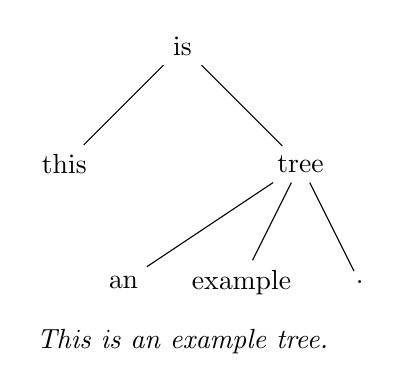
\begin{tikzpicture}
	\node (is-root) {is}
		[sibling distance=3cm]
		child { node {this} }
		child {
			node {tree}
				[sibling distance=1.5cm]
				child { node {an} }
				child { node {example} }
				child { node {.} }
				child[missing]
		};
	\path (is-root) +(0,-2.5\tikzleveldistance)
		node {\textit{This is an example tree.}};
\end{tikzpicture}

Molecular structures:
\chemfig{*6((=O)-N(-H)-(*5(-N=-N(-H)-))=-(=O)-N(-H)-)}
\chemfig{H-[1]O-[7]H}

Code snippets:

\begin{lstlisting}[language=Python]
def fibonacci_of(n):
...     if n in {0, 1}:  # Base case
...         return n
...     return fibonacci_of(n - 1) + fibonacci_of(n - 2)  # Recursive case
\end{lstlisting}

Fancy equations:

\begin{equation}\label{eq:product_decomp}
  _{s_{1}}Y_{\ell_{1} m_{1}} ~_{s_{2}}Y_{\ell_{2} m_{2}} = \sum_{S, L, M}\sqrt{\frac{(2\ell_{1}+1)(2\ell_{2}+1)}{4\pi(2L+1)}}
  \langle\ell_{1} s_{1}, \ell_{2} s_{2} | L S \rangle \langle\ell_{1} m_{1}, \ell_{2} m_{2} | LM \rangle _{S}Y_{LM}.
\end{equation}

The equations can even be embedded in-line: $\vec{F} = m \vec{a}$.

And you can also do Chemical equations:
\ce{Na2SO4 ->[H2O] Na+ + SO4^2-}

These examples are just the tip of the iceberg!

\section{Getting Started}
The best way to learn \LaTeX{} is to start using it. First we will create a document in Overleaf. Go to \url{https://www.overleaf.com}. If you've never been there before, you will see the login page. Either log-in with your account on another service, or create a new account with overleaf.

Once you have created your account, you should see your main overleaf project directory, which will look something like the screenshot (Figure~\ref{fig:home}).

\begin{figure}
\centering
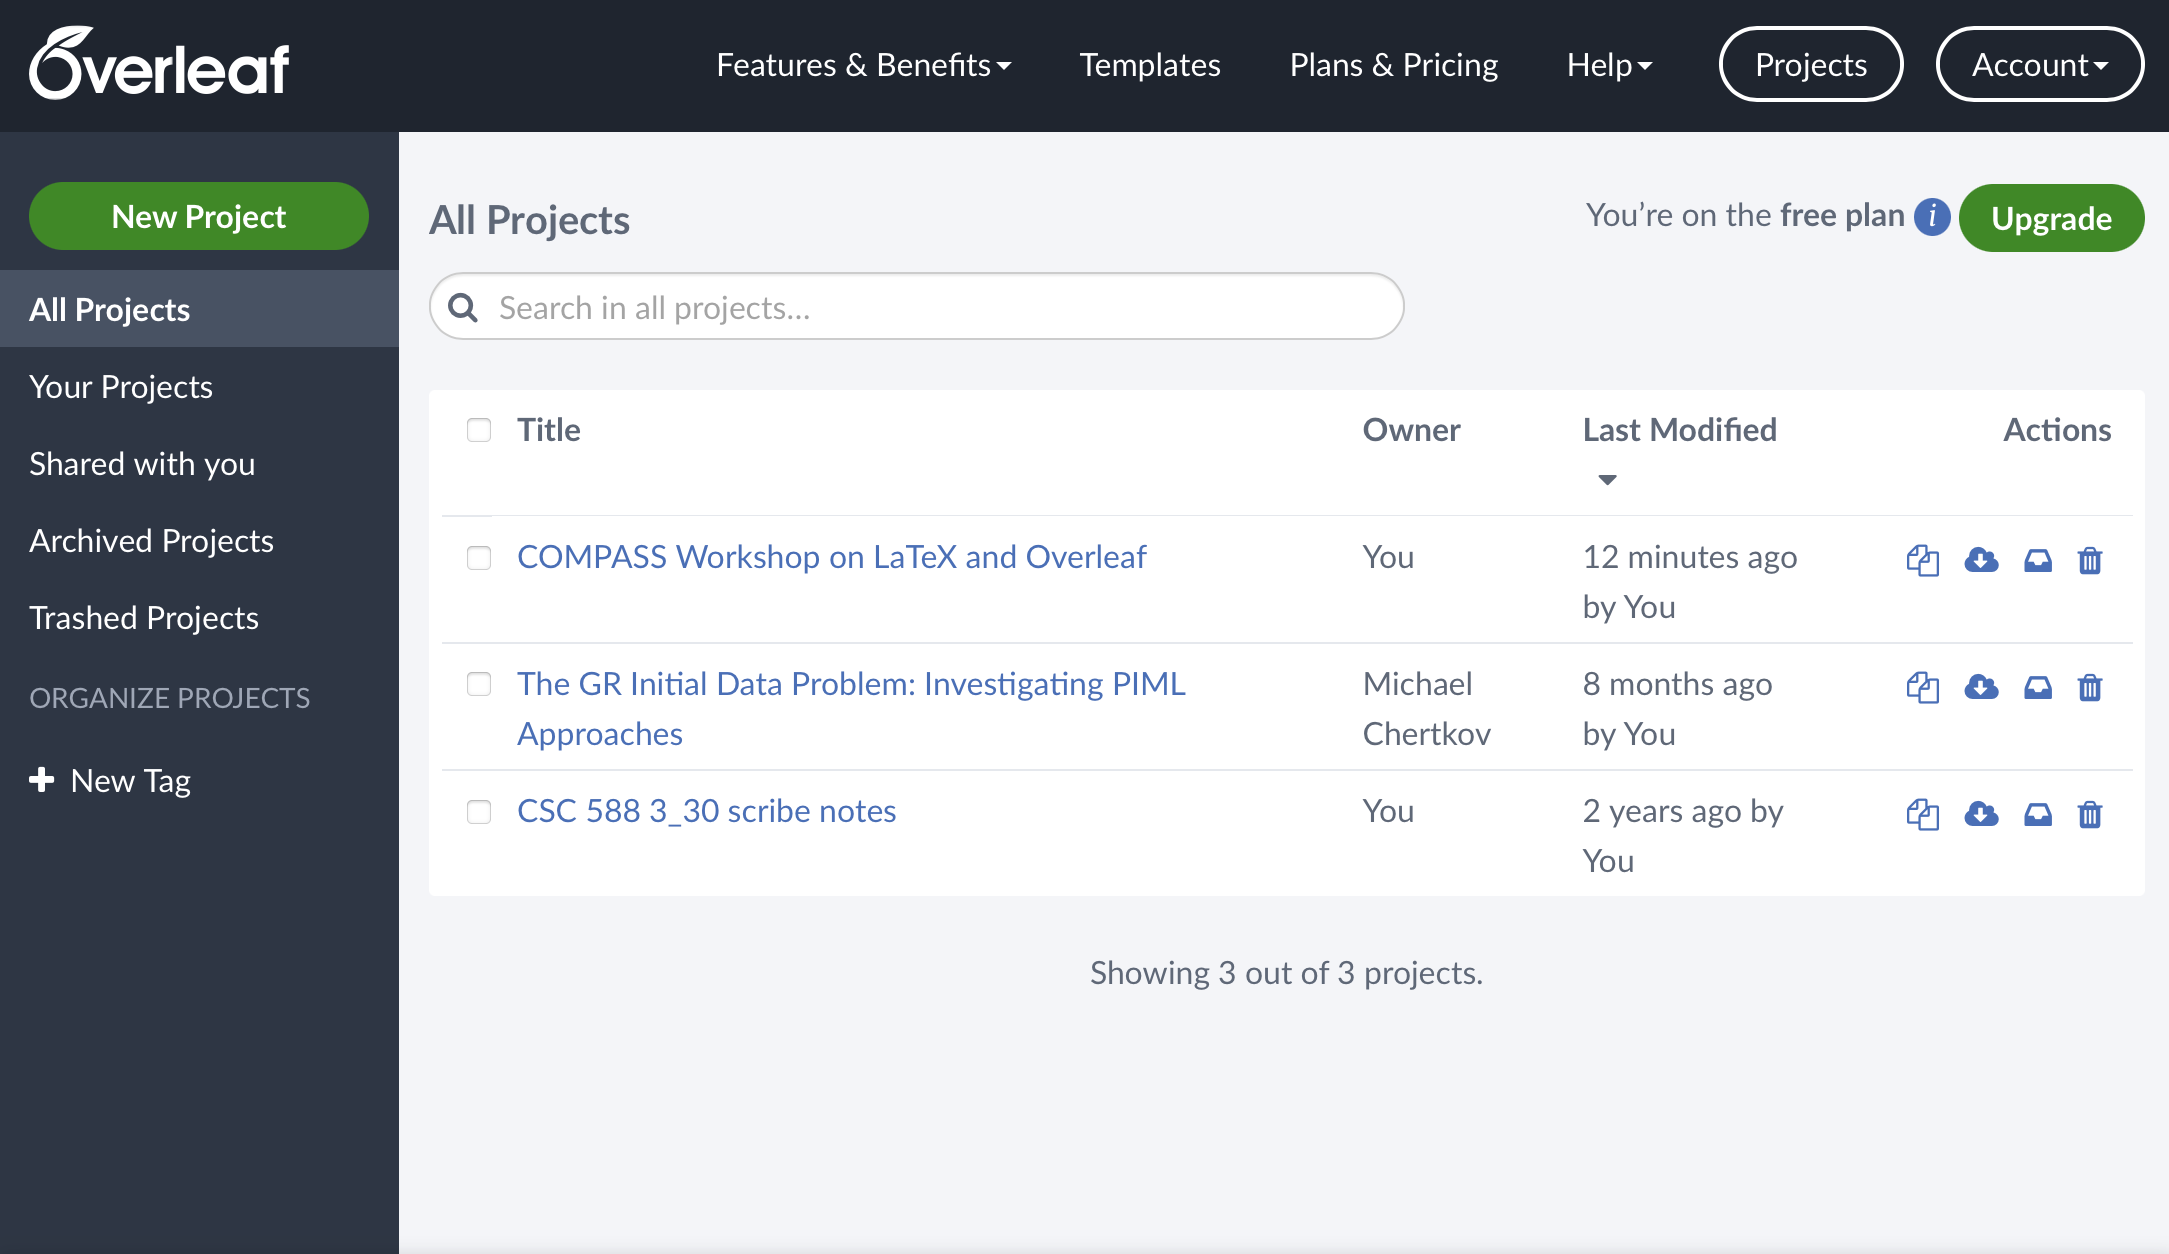
\includegraphics[width=0.75\linewidth]{Overleaf_home.png}
\caption{\label{fig:home}The home project directory of an Overleaf account.}
\end{figure}

The first thing we will do is use the new project button to create a new document. In the drop-down menu select the ``example'' option from the available templates (Figure~\ref{fig:select_example})
\begin{figure}
\centering
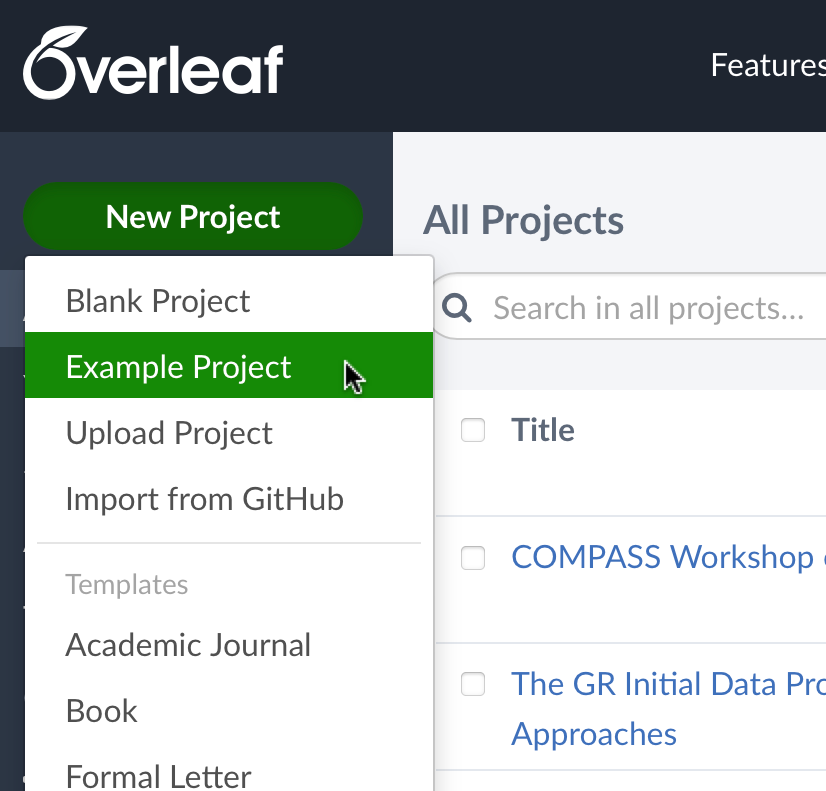
\includegraphics[width=0.5\linewidth]{select_example_project.png}
\caption{\label{fig:select_example}Select the "Example Project" template.}
\end{figure}

The document will be created and opened in Overleaf's editor. This will be a split-panel view with the document file on the left, the source code of the currently selected .tex file in the center, and the rendered document on the right.
Next, we'll read through this document to understand it.

\subsection{Basics of \TeX{}}
Lets look at the beginning of the example document. The first few lines look like this:
\begin{lstlisting}[language=TeX]
\documentclass{article}

% Language setting
% Replace `english' with e.g. `spanish' to change the document language
\usepackage[english]{babel}

% Set page size and margins
% Replace `letterpaper' with `a4paper' for UK/EU standard size
\usepackage[letterpaper,top=2cm,bottom=2cm,left=3cm,right=3cm,marginparwidth=1.75cm]{geometry}

% Useful packages
\usepackage{amsmath}
\usepackage{graphicx}
\usepackage[colorlinks=true, allcolors=blue]{hyperref}

\title{Your Paper}
\author{You}

\begin{document}
\maketitle

\begin{abstract}
Your abstract.
\end{abstract}

\section{Introduction}

Your introduction goes here! Simply start writing your document and
\end{lstlisting}
As we can see, the \TeX{} language is very simple to understand. Inside the document, plain text is the content of the document body. Back-slashes (\verb|\|) denote macros and commands. The required arguments for a command are usually surrounded by curly braces (\verb|{}|), while optional arguments use square braces (\verb|[]|). The \verb|%| symbol marks comments, which are notes to the writer that are ignored by the compiling program.

We can see that the very first command, \verb|\documentclass{article}|, sets the style of this document. This determines many of the formatting rules, fonts, page sizes, etc. You can create your own document classes, but it is often wise to use an existing one at first.

After that, there are \verb|\usepackage{}| commands. These are what unlock a lot of the magic of \LaTeX{}. Packages are collections of macros (\LaTeX{} commands) that allow you to do complex things simply. For example, here there are packages that allow language-aware formatting, adjust the paper size, enable math typsetting, and allow graphics to be embedded.

Next, the \verb|\title{}| and \verb|\author{}| commands set the title and author. It is important to realize that these commands do not draw the title! Instead, the commands just supply information about the title and author. The title is drawn once the document is made, by the \verb|\maketitle| command. Comment this command out and re-compile: the title and author will be gone. Likewise, if you attempt to call \verb|\maketitle| without the \verb|\title{}| and \verb|\author{}| set, the compilation will result in errors.

Right before the \verb|\maketitle| command, something very important happens: we begin the document, using the \verb|\begin{document}| command. The \verb|\begin{}| command is used in \LaTeX{} to signal that the block of text below it follows special rules. In this case, it follows the rules determined by the document class. Next, the abstract begins with \verb|\begin{abstract}|. This is necessary because the abstract is formatted a little differently than the rest of the document, and has special rules that need to be applied. Later on, we'll see the \verb|\begin{}| command used to start all sorts of special sections, including figures, lists, tables, equations, and code.
When the abstract is concluded, this is signaled to \LaTeX{} with the corresponding \verb|\end{abstract}| command. Not closing every \verb|\begin{}| with a corresponding \verb|\end{}| will cause an error when compiling.

Finally, we have the \verb|\section{}| command, which takes the section title as its required argument. This command starts out a section, with the text below belonging to the section until the next \verb|\section{}| command is reached. Sections can also include subsections, via the \verb|\subsection{}| command, and so on.

If we scroll all the way to the bottom of the example document, we see:

\begin{lstlisting}[language=TeX,firstnumber=110]
If you have an \href{https://www.overleaf.com/user/subscription/plans}{upgraded account}, you can also import your Mendeley or Zotero library directly as a \verb|.bib| file, via the upload menu in the file-tree.

\subsection{Good luck!}

We hope you find Overleaf useful, and do take a look at our \href{https://www.overleaf.com/learn}{help library} for more tutorials and user guides! Please also let us know if you have any feedback using the Contact Us link at the bottom of the Overleaf menu --- or use the contact form at \url{https://www.overleaf.com/contact}.

\bibliographystyle{alpha}
\bibliography{sample}

\end{document}
\end{lstlisting}
It's worth noting a few things. First, unlike the \verb|\begin{}| command, the \verb|\section{}| commands don't need a corresponding end: \LaTeX{} can figure out where the sections end, because sections only end when another section at the same level starts.

Next, we see two commands that set up the bibliography. The first, \verb|\bibliographystyle{alpha}|, chooses the style that will be used for cross-references and bibliography entries, while the second \verb|\bibliography{sample}| tells \LaTeX{} that the file named \verb|sample.bib| contains all the information for the bibliography. \verb|.bib| files are databases that collect all the citation information you need and keep it out of site. While they can be read and written by hand, it is often better to use a special tool to generate and update them, and we will be introduced to some later.

Finally, the document is ended with the \verb|\end{document}| that closes the block started by \verb|\begin{document}| near the beginning.

\subsection{More complex commands\label{section:complex}}
In the remainder of the example document, you will see examples of the commands that make,
\begin{itemize}
\item Lists
\item Tables
\item Figures
\item Equations
\item Citations
\item ... etc.
\end{itemize}
The best way to learn is to read these examples, and try making changes. The following exercises are some suggestions to try.
\subsubsection{Exercises}
\begin{enumerate}
\item In the left panel, scroll to the "How to write Mathematics" section.
\begin{itemize}
\item Notice how mathematics must be written in \textit{mathmode},

activated by \verb|$$| inline or a \verb|\begin{equation} - \end{equation}| block.
\item Add a new \textit{in-line expression} to this section: $e^{i \pi} = -1$
\item Add your own \textit{equation} to this section: $\sqrt{1+x} = 1 + \frac{1}{2}x - \frac{1}{8}x^2 \cdots$
\item Change the fractions in the existing equation so that both sides are over $2n^2$ instead of $n$.
\end{itemize}
\item Make a section of text \textit{italic} (Hint: use the buttons above the editor window)
\item Make a section of text \textit{bold}
\item Change one of the section or subsection titles.
\item Scroll to the section "How to include figures"
\begin{itemize}
\item Change the Figure caption.
\item Upload your own image and replace the existing one.
\item Make a second Figure.
\end{itemize}
\item Scroll to the "How to add lists" section
\begin{itemize}
    \item Add an item to the list
    \item Add an in-line equation to the list
    \item Look up how to make the list numbered instead of bullet-points
\end{itemize}
\item Scroll to the "How to add tables" section
\begin{itemize}
    \item Change the numbers in the table
    \item Add a new row to the table
    \item Create a second table, by copying and modifying the first one.
    \item Put an in-line equation of your choice into the table.
\end{itemize}
\end{enumerate}

If you don't know how to do something, look for an example in the document. If you can't find one, search the internet. Searching will bring up many helpful forum posts and tutorials on \LaTeX{}. There's a good chance you will find yourself back at Overleaf, because in addition to providing a document editing and collaboration system, Overleaf also provides some of the best \LaTeX{} documentation around!

This document lists many useful mathematical symbols and how to write them in \LaTeX{}: \url{http://tug.ctan.org/info/undergradmath/undergradmath.pdf}. If you can't find what you're looking for there, do a web search or try this handy website: \url{https://detexify.kirelabs.org}

Finally, because of the large number of \LaTeX{} examples and tutorials on the web, ChatGPT (and other LLMs) are pretty good at writing \LaTeX{} code as well! If you have a very specific thing you want, such as a table structured in a specific way, and aren't sure how to begin, describe what you want to a chatbot in words. It should produce well-commented code which has a good chance of compiling and doing roughly what you want. You can read it, understand how it works, and modify it as you see fit!

\subsection{References\label{section:references}}
One of the most useful features of \LaTeX{} is the ability to refer to elements by numbered references, without having to manually assign the numbers. When writing the document you assign a named label to the element you want to references using the \verb|\label{}| command, then you can refer to that label again with the \verb|\ref{}| command. For example, I can refer to subsection~\ref{section:complex} by placing this label in its title:
\begin{lstlisting}[language=TeX,firstnumber=148]
\subsection{More complex commands\label{section:complex}}
\end{lstlisting}
Then calling \verb|\ref{section:complex}| when I need the section number. Or I can write an equation,

\begin{equation}\label{eq:rel_energy_momentum}
E^2 = p^2 c^2 + m^2 c^4.
\end{equation}
And then I can reference the equation above as Equation~\ref{eq:rel_energy_momentum} by doing this:

\begin{lstlisting}[language=TeX,firstnumber=172]
\begin{equation}\label{eq:rel_energy_momentum}
E^2 = p^2 c^2 + m^2 c^4.
\end{equation}
And then I can reference the equation above as Equation \ref{eq:rel_energy_momentum} by doing this:...
\end{lstlisting}
Note that starting the reference labels with "\verb|eq:|" and "\verb|section:|" is not necessary, it's just a nice convention to follow to keep the types of references straight.

\textbf{Exercise:} Try it in your own document!

\subsection{Citations and BibTex files}
We saw from the example document that citations in \LaTeX{} require a bibliography file with a .bib extension--called a BibTex file. Here, we'll delve into what those files do, and how to produce them.

\subsubsection{Reading BibTex files}
The first thing to know about BibTex files is that they are human readable. Go ahead and open the one from the sample document, you will see this:
\begin{lstlisting}[language=TeX]
@article{greenwade93,
    author  = "George D. Greenwade",
    title   = "The {C}omprehensive {T}ex {A}rchive {N}etwork ({CTAN})",
    year    = "1993",
    journal = "TUGBoat",
    volume  = "14",
    number  = "3",
    pages   = "342--351"
}
\end{lstlisting}
As indicated by the different extension, this file is not in the \TeX{} language, although it is closely related. The \verb|@article{...}| block defines a database entry describing the metadata for an article. Within the entry, we can see that properties needed for the bibliography, such as the author, title, year, etc. are all provided.

At the beginning of the entry there is a piece of information with no associated field: \verb|greenwade93|. This defines the label that will be used to cite the article in the text. This label is never seen by the end reader, so it doesn't need to be pretty. But it does need to be memorable for you, the writer, because this is how you will cite that paper. In the main .tex file, you will see the citation is created by the command \verb|\cite{greenwade93}|. This creates a mark in the text, but this mark isn't the label we see in the .tex file, instead, it is determined by the citation style setting \verb|\bibliographystyle{alpha}|. Try changing this to \verb|\bibliographystyle{unsrt}| and recompiling. Or, say you want something more like APA: in that case, try \verb|\bibliographystyle{apalike}|.

\subsubsection{Writing BibTex files}
The second thing you should know about .bib files is that they are human writable. Given the example above, go ahead and add a second reference into the bibliography--just make something up. Once the reference exists, you can cite it in your text. If you don't cite it, not only will a marker for it not appear in the body of the text, but it also won't appear in the bibliography: \textit{the bibliography only shows entries from the .bib file that have been cited}.

\subsubsection{Managing BibTex files}
The third thing you should know about .bib files, is that humans shouldn't read or write them! They are database files, the domain of machines. It is far easier, and better practice, to use special software tools to create the .bib files for your research.

One stand-alone, cross-platform tool that can do this is JabRef (\url{https://www.jabref.org}). This program creates and views .bib files in a graphical interface. Most usefully, JabRef is very good at pulling all the needed information for a .bib entry off of the internet! Just pasting a DOI link or other reference typically is enough to automatically generate the whole entry.

A more involved option is to use Zotero (\url{https://www.zotero.org}). Zotero is an extremely useful application for managing your research sources. You can create many collections of references, store your annotated files, notes, and biblographic metadata all in one place. Zotero comes with a browser extension that allows you to create a library entry from whatever page you are looking at in your browser: automatically retrieving the publication information and downloading the text if it can find it. But what makes this work really well with \LaTeX{} is a Zotero extension called Better BibTex (\url{https://retorque.re/zotero-better-bibtex/}). Better BibTex allows you to export .bib files from Zotero that are based on the metadata Zotero has collected. This allows you to instantly make your Zotero library citable from any \LaTeX{} project, and you can even set up a .bib file to be continuously synced whenever you make changes to the associated Zotero library.

\subsection{\LaTeX{} Challenges}
Test your ability to figure out how to do stuff in \LaTeX{} with these \textbf{\textit{challenge questions}}!
\begin{itemize}
\item Figure out how to make a multi-line equation and reference the individual lines.
\item Add an appendix to the document.
\item Add a table of contents to the document.
\item Look up how to get rid of the section numbers and try to do that.
\item Embed a snipped of code in the document with automatic syntax highlighting and line numbering.
\item Try writing these crazy equations from my research!
\end{itemize}

\begin{equation}\label{eq:stress_eng_consrv}
  \nabla_{\mu}\left( \int d\Omega n^{\gamma} n^{\mu} I \right) = \int d\Omega n^{\gamma}(j - \alpha I).
\end{equation}

\begin{subequations}\label{eq:rt_cov_sph2}
  \begin{align}
    \nabla_{\mu}\left( \frac{n^{\mu} I_{\nu}}{\nu} \right)
    &+ \frac{\partial}{\partial \nu}\left(-n^{A}n^{B}\omega^{I}_{AB} n_{I} I_{\nu} \right) \\
    &+ \frac{1}{\sin{(\theta)}}\frac{\partial}{\partial \theta}\left( \sin{(\theta)} (-n^{A}n^{B}((\cos{\phi}\omega^{X}_{AB}+\sin{\phi}\omega^{Y}_{AB})\cos{\theta} - \sin{\theta}\omega^{Z}_{AB}) ) \frac{I_{\nu}}{\nu} \right) \\
    &+\frac{\partial}{\partial \phi}\left((-n^{A}n^{B}(\cos{\phi}\omega^{Y}_{AB} - \sin{\phi}\omega^{X}_{AB})\frac{1}{\sin{\theta}} ) \frac{I_{\nu}}{\nu} \right) = \frac{j_{\nu} - \alpha_{\nu}I_{\nu}}{\nu}.
  \end{align}
\end{subequations}

\section{Collaboration via Overleaf\label{section:sharing}}
On overleaf it is possible for multiple authors to share and collaborate on a document.
Simply click the "share" button at the top of the screen. The sharing window will pop up (Figure~\ref{fig:share}). The options are pretty self-explanatory, and not too different from Google Docs.

\begin{figure}
\centering
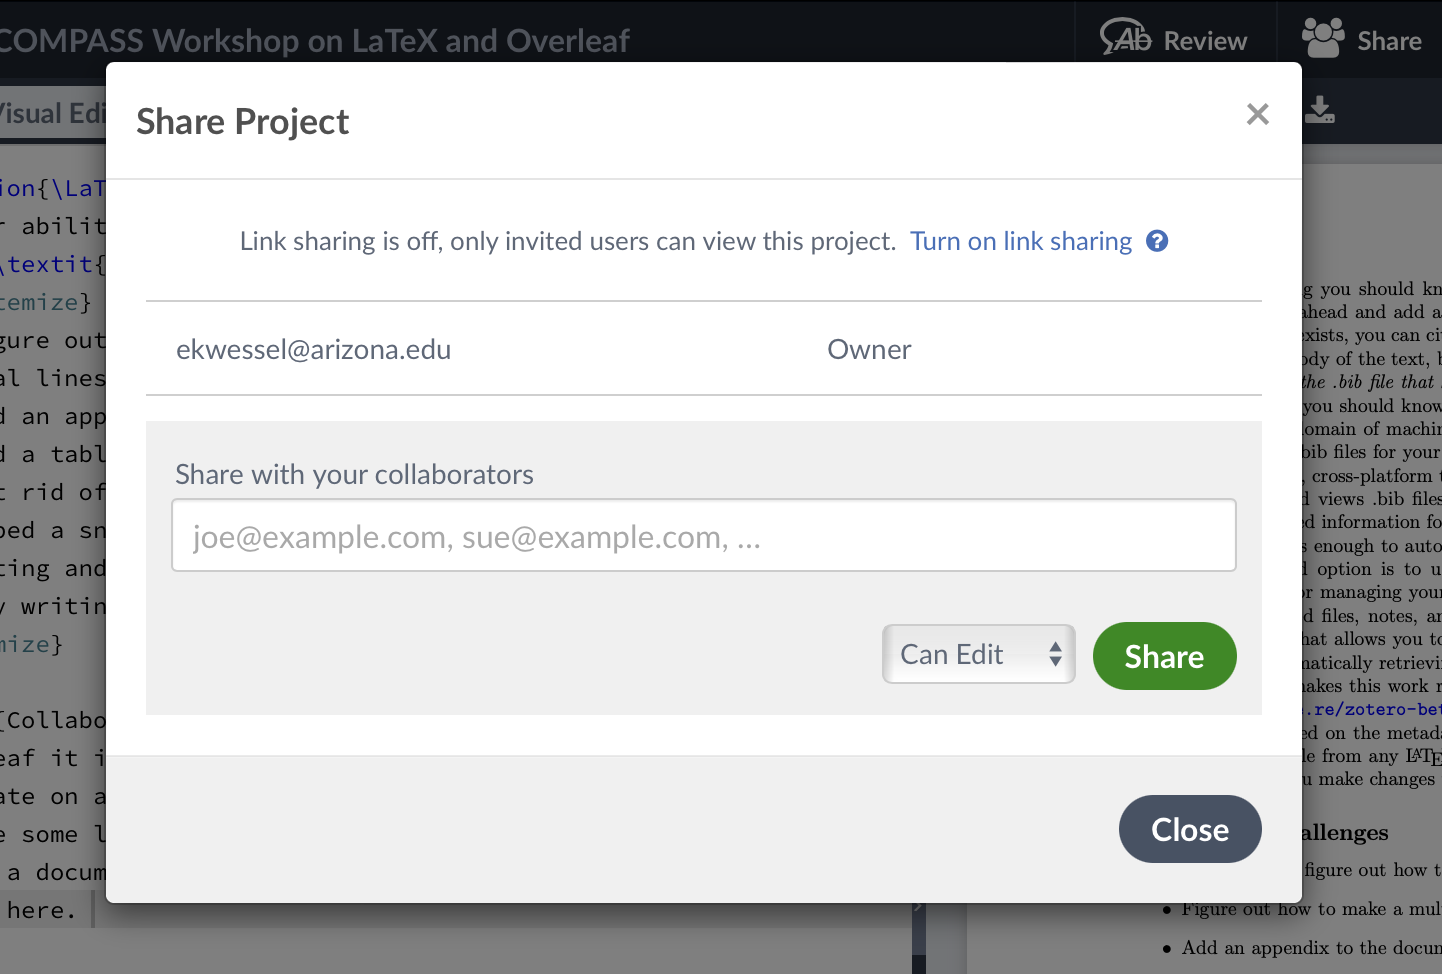
\includegraphics[width=0.75\linewidth]{share.png}
\caption{\label{fig:share}The Overleaf project sharing panel.}
\end{figure}

Unfortunately, free accounts are limited in the number of collaborators they can have. The only way to have more than one collaborator is to work with someone who has one of the paid plans. The details can be found here \url{https://www.overleaf.com/user/subscription/plans}.

\section{Advanced Topics}

\subsection{Using \LaTeX{} without Overleaf}
We saw in section~\ref{section:sharing} that Overleaf charges for using it's collaboration features for more than one person, which is definitely an inconvenience.

However, there is a way around this problem. \LaTeX{} is \textit{free software}, it existed long before Overleaf, and we don't need to be dependent on it to us \LaTeX{}! It is possible to install \LaTeX{} compilers on your own machine. Because \LaTeX{} is essentially \textit{source code} for your documents, you can edit it with any tool you use to edit code: Vim, Emacs, Sublime Text, VSCode, even jupyter if you want to be crazy! Or, you can download a special purpose \LaTeX{} editor, there are several to choose from.

Then, if you want to collaborate with someone else, you can do so the way you collaborate on code by creating a git repository on GitHub or Bitbucket.

The key to doing this is getting \LaTeX{} on your machine. There are several options depending on your platform:
\begin{itemize}
    \item Linux - TBD
    \item Mac - TBD
    \item Windows -TBD
\end{itemize}

\subsection{Defining your own macros}
TBD.

\subsection{Creating your own document class}
TBD.

\end{document}